\documentclass[11pt]{article}
\usepackage{graphicx}
\graphicspath{ {./images/} }

\usepackage{amsmath}
\usepackage{textcomp}
\usepackage[top=0.8in, bottom=0.8in, left=0.8in, right=0.8in]{geometry}
% Add other packages here %
\usepackage{indentfirst}
\usepackage{float}
\usepackage[usenames, dvipsnames]{color}

% Put your group number and names in the author field %
\title{\bf Excercise 1.\\ Implementing a first Application in RePast: A Rabbits Grass Simulation.}
\author{Group \textnumero{44}: Cyril Van Schreven, Valentin Kindschi}

\begin{document}
\maketitle

\section{Implementation}

\subsection{Assumptions}
% Describe the assumptions of your world model and implementation (e.g. is the grass amount bounded in each cell) %

There are 200 grass energy in the beginning of the simulation, each cell having between 0 and 32 points. The grass can randomly grow over existing grass cell up to 32 points. The rabbits start with 15 energy and the price to reproduce is of 7 energy points. All the other parameters (grid size, initial number of rabbits, energy needed to reproduce and grass amount added in each step) can be set by the user.


\subsection{Implementation Remarks}
% Provide important details about your implementation, such as handling of boundary conditions %

When looking for an appropriate cell to place a new rabbit: we pick a random cell and look whether it is available. If it is not, we try again. We assume that if 10*width*height attempts fail (that is 4000 for a 20x20 grid), there is no cell available. Thus, the rabbit is not added.

When a rabbit plans to move to a cell where there is already a rabbit, he cancels his action and does not move for that step. He does nevertheless eat the grass under him.

The space has no borders, which means that if a rabbit cross the upper boundary, it will appears at the bottom of the space. Same for the left and right borders.

The cost of reproducing is of 7 energy.

\section{Results}

% In this section, you study and describe how different variables (e.g. birth threshold, grass growth rate etc.) or combinations of variables influence the results. Different experiments with diffrent settings are described below with your observations and analysis

%Default unaffected settings:   private static final int NUMRABBITS = 10;
% WORLDXSIZE = 20;
% WORLDYSIZE = 20;
% BIRTHTHRESHOLD = 50;
% GRASSGROWTHRATE = 20;
% INITIALGRASS = 200;
% RABBITINITIALENERGY = 15;
% BIRTHENERGYCOST = 7;

\subsection{General observation}
With a set of reasonable parameters, the population of rabbits or grass will evolve according to a certain pattern. First, there is not enough grass for the rabbits to survive and most of them die. Then the grass can grow without being eaten and the total amount increases. The surviving rabbits can then gain energy and reproduce. The rabbit population increases until it reaches a peak where there is not enough grass for them to survive. The system is back in its first step and repeats. As the cycle continues, the lows and high are less far apart. On the population plot of the rabbits and grass this results in a damped oscillation. 

Now, we can study how changing the parameters may affect the average value of these oscillations and their amplitude. \textbf{On the following figures, the number of rabbits are shown in \textcolor{blue}{blue}, while the total amount of grass is in \textcolor{red}{red}.}

\subsection{Experiment 1}
% The effect of grass growth rate
The goal of the first experiment is to analyze the effect of the grass growth rate on the amount of grass and number of rabbits. The other parameters are fixed.

\subsubsection{Settings}

\begin{table}[H]
\centering
\begin{tabular}{|l|c||l|c|}
\hline
Grid size         & 20 x 20             & Birth threshold           & 50 \\ \hline
Grass growth rate & \textit{variable}   & Initial number of rabbits & 10 \\ \hline
\end{tabular}
\caption{Settings for the experiment 1}
\end{table}

\subsubsection{Observations}
% Elaborate on the observed results %

\begin{figure}[H]
	\centering
	\begin{minipage}{0.49\linewidth}
    	\centering
    	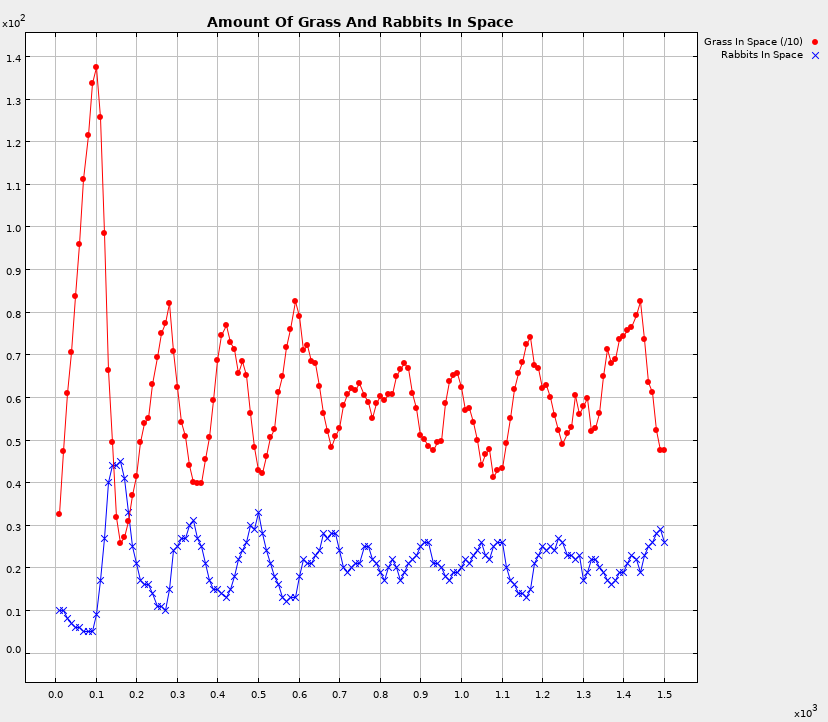
\includegraphics[scale = 0.2]{plot_snapshot_exp1_ggr=20}
    	\caption{Grass growth rate = 20}
        \label{fig:ggr20}
	\end{minipage}
    	\begin{minipage}{0.49\linewidth}
    	\centering~
    	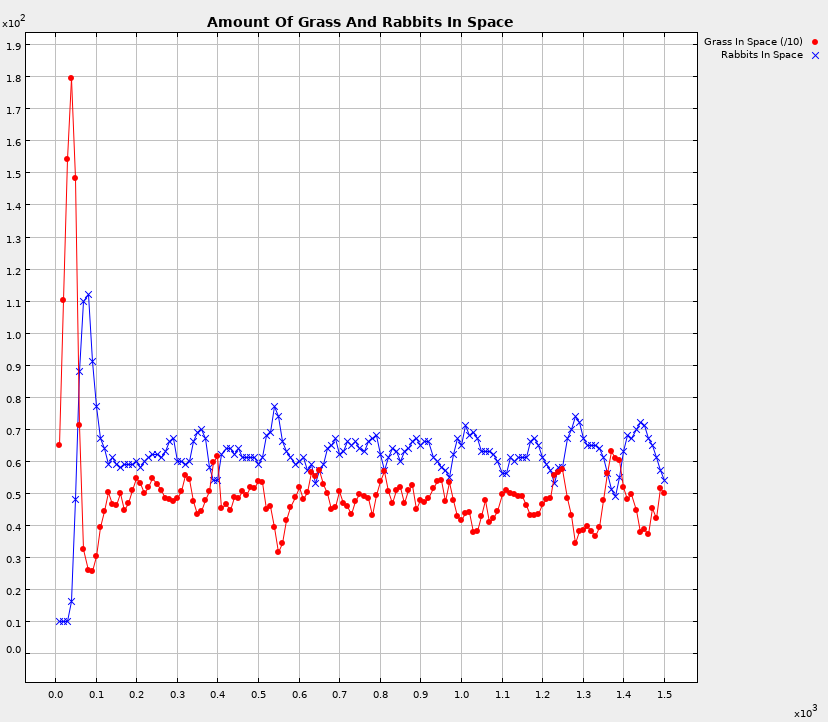
\includegraphics[scale = 0.2]{plot_snapshot_exp1_ggr=60}
    	\caption{Grass growth rate = 60}
        \label{fig:ggr60}
	\end{minipage}
\end{figure}

As one can see on Fig. (\ref{fig:ggr20}) with a grass growth rate of 20 per step, the average amount of grass in space oscillates around 600 and the average number of rabbits is around 20. On the second figure, with a grass growth rate of 60 per step, the average amount of grass in space is slightly lower, at 500. The average number of rabbits is significantly higher: around 60. 

Thus, increasing the growth rate of the grass helps the rabbit population. Because of the growth of the rabbit population, it also indirectly has a negative effect on the total amount of grass in space.

A second aspect to observe is that with less grass growth, the oscillations of both population are stronger. What happens is that when the total amount of grass is low, the rabbit population will radically decrease (by a factor of two approximately). When the grass growth is higher, the rabbit population will not suffer as much from it.

\subsection{Experiment 2}
% The effect of birth threshold
The goal of the second experiment is to find the effect of the rabbit's birth threshold parameter on the amount of grass and number of rabbits.

\subsubsection{Settings}

\begin{table}[H]
\centering
\begin{tabular}{|l|c||l|c|}
\hline
Grid size         & 20 x 20 & Birth threshold           & \textit{variable}  \\ \hline
Grass growth rate & 20      & Initial number of rabbits & 10                 \\ \hline
\end{tabular}
\caption{Settings for the experiment 2}
\end{table}

\subsubsection{Observations}
% Elaborate on the observed results %
%Higher birth threshold: more stability; less oscillations%

\begin{figure}[H]
	\centering
	\begin{minipage}{0.49\linewidth}
    	\centering
    	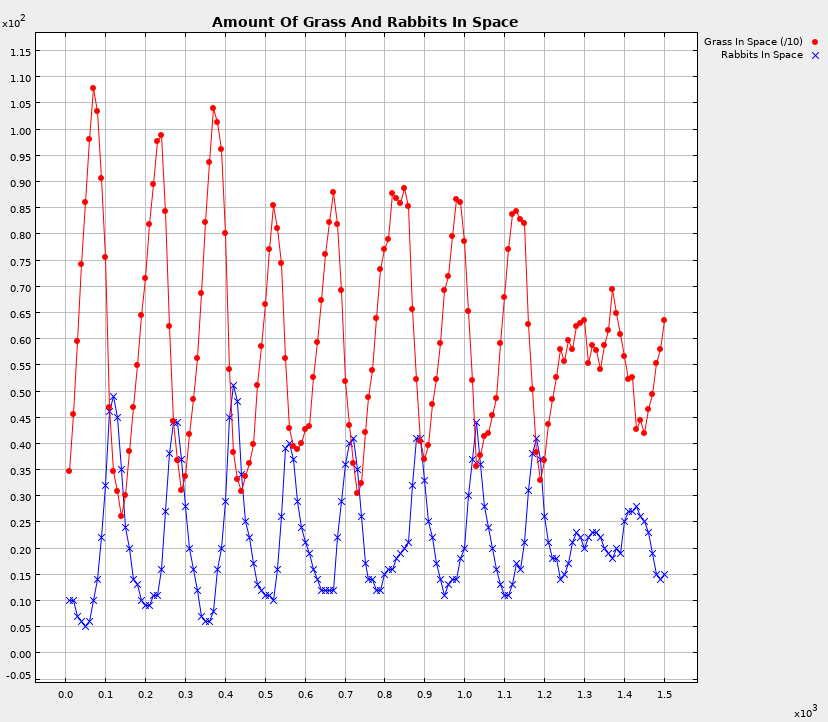
\includegraphics[scale = 0.2]{plot_snapshot_exp2_bt=35}
    	\caption{Birth threshold = 35}
        \label{fig:bt35}
	\end{minipage}
    	\begin{minipage}{0.49\linewidth}
    	\centering~
    	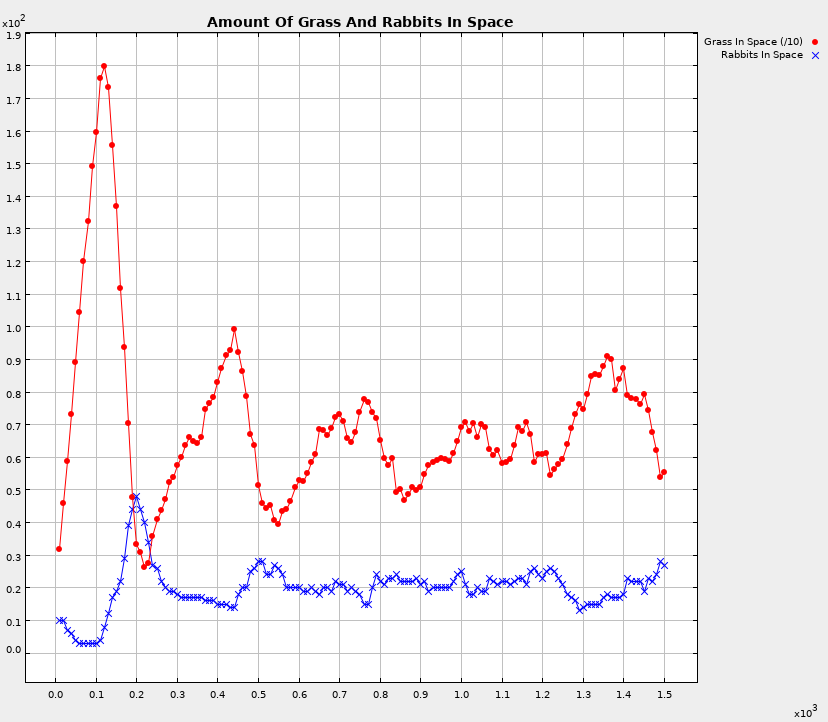
\includegraphics[scale = 0.2]{plot_snapshot_exp2_bt=100}
    	\caption{Birth threshold = 100}
        \label{fig:bt100}
	\end{minipage}
\end{figure}

With a birth threshold of 35 (Fig. (\ref{fig:bt35})), there are extremely high oscillations. The rabbit population will reproduce a lot when possible, and then die due to lack of grass. With this set-up the rabbits would even go extinct during some simulations. With a birth threshold of 100 however, the number of rabbits alive is very stable (Fig. (\ref{fig:bt100})). The total amount of grass varies but this is mostly due to randomness. This setup is more stable for the rabbits population because some rabbits with higher energy exist and can thus sustain even when grass is lacking.\\

Increasing or decreasing the birth threshold does not, however, affect the average number of rabbits or the average amount of grass in a noticeable way.


\subsection{Experiment 3}
% The effect of grid size
Finally, the last experiment consists in observing the impact of the grid size on the amount of grass and number of rabbits.

\subsubsection{Settings}

\begin{table}[H]
\centering
\begin{tabular}{|l|c||l|c|}
\hline
Grid size         & \textit{variable}   & Birth threshold           & 50    \\ \hline
Grass growth rate & 20                  & Initial number of rabbits & 10    \\ \hline
\end{tabular}
\caption{Settings for the experiment 3}
\end{table}

\subsubsection{Observations}
% Elaborate on the observed results %
As expected, changing the initial number of rabbits will not affect the steady-state. It will affect the initial conditions and thus the first oscillations. If the number of rabbits is high, the majority of rabbits will die soon. The system will start with strong oscillations. On the contrary, if there are only a couple of rabbits in the beginning, assuming that they survive, the oscillations will be soft and the steady-state will be reached much faster.

\end{document}